% Copyright 2022 Haute école d'ingénierie et d'architecture de Fribourg
%
% Licensed under the Apache License, Version 2.0 (the "License");
% you may not use this file except in compliance with the License.
% You may obtain a copy of the License at
%
% http://www.apache.org/licenses/LICENSE-2.0
%
% Unless required by applicable law or agreed to in writing, software
% distributed under the License is distributed on an "AS IS" BASIS,
% WITHOUT WARRANTIES OR CONDITIONS OF ANY KIND, either express or implied.
% See the License for the specific language governing permissions and
% limitations under the License.

% =============================================================================
% | HES-SO//Master - Thesis project report template                           |
% |                                                                           |
% | Originally based on the EPFL template, with many adjustments             |
% =============================================================================

% Document settings
\documentclass[a4paper,11pt,fleqn]{book}
\usepackage[utf8]{inputenc}
\usepackage[T1]{fontenc}
\usepackage[english]{babel}



% -----------------------------------------------------------------------------
% Preamble
% -----------------------------------------------------------------------------
% =============================================================================
% | Thesis metadata                                                           |
% =============================================================================

% Thesis info
\newcommand{\ThesisTitle}{GPU optimization - Celeritas}
\newcommand{\ThesisSubject}{}
\newcommand{\Orientation}{Information and communication systems (ICS) }
\newcommand{\Keywords}{}
\newcommand{\Keywordsfr}{}
\newcommand{\reportVersion}{v0.1}
\newcommand{\specificationVersion}{v1.3}

% Author
\newcommand{\AuthorFirstName}{Simon }
\newcommand{\AuthorLastName}{Barras}
\newcommand{\Author}{\AuthorFirstName \AuthorLastName}

% Advisor
\newcommand{\AdvisorFirstName}{Frédéric }
\newcommand{\AdvisorLastName}{Bapst}
\newcommand{\AdvisorSchool}{HEIA-FR}
\newcommand{\Advisor}{Prof. \AdvisorFirstName \AdvisorLastName}
\newcommand{\AdvisorTwoFirstName}{Jean }
\newcommand{\AdvisorTwoLastName}{Hennebert}
\newcommand{\AdvisorTwoSchool}{HEIA-FR}
\newcommand{\AdvisorTwo}{Prof. \AdvisorTwoFirstName \AdvisorTwoLastName}
\newcommand{\Expert}{Dr. Baptiste Wicht}

% Mendant
\newcommand{\Mendant}{\acrfull{lbl}\\ & Paolo Calafiura\\ & Julien Esseiva}

% Place (for date and place)
\newcommand{\Date}{\today}
\newcommand{\Place}{Berkeley, CA, USA}
         % your project data
% ==================
% Template settings
% ==================

% General tools
% -------------
\usepackage{etoolbox}
\usepackage{listings}

% Page style
% ----------
\usepackage[margin=3cm, left=3.5cm, right=3.5cm, twoside=false]{geometry}
\usepackage{fancyhdr}
\setlength{\headheight}{14pt}
\renewcommand{\sectionmark}[1]{\markright{\thesection\ #1}}
\pagestyle{fancy}

% Standard pages (inside chapters)
\fancyhf{}
\renewcommand{\headrulewidth}{0.4pt}
\renewcommand{\footrulewidth}{0.4pt}
\fancyhead[R]{\bfseries \nouppercase{\rightmark}}
\fancyhead[L]{\bfseries \nouppercase{\leftmark}}
\fancyfoot[L]{\Author \space - \ThesisTitle}
\fancyfoot[R]{\thepage}

% First page of chapters
\fancypagestyle{plain}{
	\fancyhf{}
	\renewcommand{\headrulewidth}{0pt}
	\fancyfoot[L]{\Author \space - \ThesisTitle}
	\fancyfoot[R]{\thepage}
}

% Imports for external PDFs
\fancypagestyle{addpagenumbersforpdfimports}{
	\fancyhead{}
	\renewcommand{\headrulewidth}{0pt}
	\fancyfoot{}
	\fancyfoot[R]{\thepage}
}

% Use empty style for page when clearing double pages
%\def\cleartoodd{%
%	\clearpage%
%	%\ifodd\value{page}\else\mbox{}\thispagestyle{empty}\newpage\fi%
%}

%\def\clearchap{%
%	\ifodd\value{page}\else\mbox{}\thispagestyle{empty}\fi%
%}

% \cleardoublepage replaced by \cleartoodd
%\let\origdoublepage\cleardoublepage
%\renewcommand{\cleardoublepage}{%
%	\cleartoodd%
%}

% Fonts
% -----

% Helvetica (Arial used in the MSE Word template)
\usepackage{helvet}
\usepackage{lmodern}
\usepackage[T1]{fontenc}


% Math
% ----
\usepackage{amsmath}  % better math

% Floats and figures
% ------------------
\usepackage{newfloat}          % floats
\usepackage[oneside]{caption}  % captions
\usepackage{subcaption}        % subcaptions
\usepackage[section]{placeins} % allows to put float barriers

% Float captions in italics, with the label in the margin
%\DeclareCaptionLabelFormat{title}{#1 #2}
%\DeclareCaptionLabelFormat{hangout}{\llap{#1 #2\hspace{5mm}}}
%\captionsetup{
%	format=hang,
%	labelformat=hangout,
%	singlelinecheck=false,
%	font={it}
%}

% Caption with a source for a figure
% TODO: improve this to use square brackets like the normal "caption"
\newcommand*{\captionsource}[3]{%
	\caption[{#1}]{%
		#2%

		\textbf{Source:} #3%
	}%
}

% Tables
% ------
\usepackage{booktabs} % much better tables
\usepackage{multirow} % allows to fuse rows
\usepackage{array}    % manipulate array
\usepackage{tabularx} % better tables

% Define new tabularx column types:
%  - R: streteched right-aligned
%  - C: stretched centered
%  - N: left aligned, specified space
\newcolumntype{R}{>{\raggedleft\arraybackslash}X}%
\newcolumntype{C}{>{\centering\arraybackslash}X}%
\newcolumntype{N}[1]{>{\raggedleft\arraybackslash}p{#1}}

% Set row height multiplicator to provide more breathing space
\renewcommand{\arraystretch}{1.3}

% Bibliography
% -------------------

% Use biber, with numeric style and no sorting (citation order)
\usepackage[
backend=biber,
style=numeric,
sorting=none,
bibencoding=auto
]{biblatex}
\addbibresource{bibliography.bib}


% Tables of contents, figures, tables and listings
% ------------------------------------------------
\usepackage{tocloft}
\newlistof{listing}{lol}{List of Listings}
\setcounter{tocdepth}{1} % Depth to 'section'
\setlength{\cftfigindent}{0pt}  % remove indentation from figures in lof
\setlength{\cftfignumwidth}{1cm}
\setlength{\cfttabindent}{0pt}  % remove indentation from tables in lot
\setlength{\cfttabnumwidth}{1cm}
\setlength{\cftlistingindent}{0pt}
\setlength{\cftlistingnumwidth}{1cm}

% Mini tables of contents
% -----------------------
\usepackage{minitoc}

% no "Contents" title
\mtcsettitle{minitoc}{Contents}

% Layout
\setlength{\mtcindent}{-0.5em}
\mtcsetoffset{minitoc}{-1em}

% Spacing above and below table
\mtcsetfeature{minitoc}{before}{\vspace{0.5cm}}
\mtcsetfeature{minitoc}{after}{\vspace{-0.25cm}}
\renewcommand{\mtifont}{\sffamily\bfseries\large}

% Colors & graphics
% -----------------
\usepackage[table]{xcolor}    % colors
\usepackage[pdftex]{graphicx} % graphics importing
\graphicspath{{02-main/figures/}}
\definecolor{gray80}{gray}{0.80}


% Code and syntax highlighting
% ----------------------------
\usepackage[newfloat]{minted}   % code highlighting
\newenvironment{code}{\captionsetup{type=listing}}{}

% Typography
% ----------
\usepackage{csquotes}                    % paragraph indentation and spacing
\usepackage[defaultlines=3,all]{nowidow} % avoid widows and orphans
\usepackage{microtype}                   % typographic improvements
\usepackage{parskip}                     % No indent and auto-space between paragraphs
\usepackage[super]{nth}
\usepackage{amsmath}

\usepackage{paralist}
\usepackage{enumitem}
\setlist{after=\vspace{\baselineskip}}

% Section and chapters headings
% -----------------------------
\usepackage[explicit]{titlesec} % titles formatting
%\usepackage{titletoc} % titles formatting in ToC etc
%\usepackage{sectsty}  % sectioning commands

% -- Chapters --
% Remove "Chapter N" and use a sans-serif font

% Set layout lengths
\setlength{\headheight}{8mm}
\setlength{\footskip}{1.5cm}
\addtolength{\textheight}{-.5cm}

\titlespacing{\chapter}{-5mm}{-10mm}{3mm}
\titlespacing{\section}{-5mm}{3mm}{2mm}
\titlespacing{\subsection}{-5mm}{2mm}{2mm}
\titlespacing{\subsubsection}{-5mm}{2mm}{1mm}


%\titleformat{\chapter}[block]
%{\Huge}
%{\thechapter\hspace{12pt}\textcolor{gray80}{|}\hspace{12pt}}
%{0pt}
%{\Huge\bfseries}

\titleformat{\chapter}{\Huge\bfseries}{\llap{\thechapter\hspace{12pt}\textcolor{gray80}{|}}}{0mm}{%
	\hfill\begin{minipage}[t]{\dimexpr\textwidth}\raggedright#1\end{minipage}%
}
\titleformat{\section}{\Large\bfseries}{\llap{\thesection}}{0mm}{%
	\hfill\begin{minipage}[t]{\dimexpr\textwidth}\raggedright#1\end{minipage}%
}
\titleformat{\subsection}{\large \bfseries}{\llap{\thesubsection}}{0mm}{%
	\hfill\begin{minipage}[t]{\dimexpr\textwidth}\raggedright#1\end{minipage}%
}
\titleformat{\subsubsection}{\bfseries}{\llap{\thesubsubsection}}{0mm}{%
	\hfill\begin{minipage}[t]{\dimexpr\textwidth}\raggedright#1\end{minipage}%
}

% Misc
% ------
\usepackage{lipsum}    % filler text
\usepackage{blindtext} % random text
\usepackage{lscape}    % easy landscape pages
\usepackage{pdflscape} % landscape pages for PDFs

% Allow email typesetting
\newcommand{\email}[1]{%
	\href{mailto:#1}{\textit{#1}}%
}

% References
% -----------
\usepackage{url}

% pdf metadata
\usepackage[
	pdfauthor={\Author},
	pdftitle={\ThesisTitle},
	pdfsubject={\ThesisSubject},
	pdfkeywords={\Keywords}
	pdfduplex=DuplexFlipLongEdge]{hyperref}

% Hyperlinks
\hypersetup{
	colorlinks=true,
	linkcolor=black,
	citecolor=black,
	filecolor=black,
	urlcolor=black,
}
\providecommand*{\listingautorefname}{Listing}


% % Glossary
% % --------
%\usepackage[xindy, toc, nonumberlist]{glossaries}
\usepackage[acronym]{glossaries}
\makeglossaries
\newacronym{heia}{HEIA-FR}{Haute Ecole d'Ingénierie et d'Architecture de Fribourg}

\newacronym{os}{OS}{Operating System}

\newacronym{gpu}{GPU}{Graphics Processing Unit}

\newacronym{cpu}{CPU}{Central Processing Unit}

\newacronym{cuda}{CUDA}{Compute Unified Device Architecture}

\newacronym{lbl}{LBNL}{Lawrence Berkeley National Laboratory}

\newacronym{ornl}{ORNL}{Oak Ridge National Laboratory}

\newacronym{anl}{ANL}{Argonne National Laboratory}

\newacronym{fnal}{FNAL}{Fermi National Accelerator Laboratory}

\newacronym{bnl}{BNL}{Brookhaven National Laboratory}

\newacronym{cern}{CERN}{European Organization for Nuclear Research}

\newacronym{lhc}{LHC}{Large Hadron Collider}

\newacronym{doe}{DOE}{Department of Energy}

\newacronym{smart}{SMART}{Specific, Measurable, Achievable, Relevant, Time-bound}

\newacronym{hpc}{HPC}{High Performance Computing}

\newacronym{nersc}{NERSC}{National Energy Research Scientific Computing Center}

\newacronym{atlas}{ATLAS}{A Toroidal LHC ApparatuS}

\newacronym{cms}{CMS}{Compact Muon Solenoid}

\newacronym{hep}{HEP}{High Energy Physics}

\newacronym{rkdp}{RKDP}{Runge Kutta Dormand Prince}

\newacronym{simd}{SIMD}{Single Instruction Multiple Data}

\newacronym{sisd}{SISD}{Single Instruction Single Data}

\newacronym{sm}{SM}{Streaming Multiprocessor}

\newacronym{sdk}{SDK}{Software Development Kit}

\newacronym{api}{API}{Application Programming Interface}

\newacronym{simt}{SIMT}{Single Instruction Multiple Thread}



\usepackage{tabularray}    % template settings
% ===========================================
% = Codestyles for minted syntax highlighting
% ===========================================


% How to use (replace 'java' with language name):
% - code blocks:
%     \begin{javacode}
%     CODE
%     \end{javacode}
% - files:
%     full: \javafile{PATH}
%     extract: \javafile[startline=x, endline=y]{PATH}

% c#
\newminted{csharp}{frame=single, framesep=6pt, breaklines=true, fontsize=\scriptsize}
\newmintedfile{csharp}{frame=single, framesep=6pt, breaklines=true,
fontsize=\scriptsize}

% Java
\newminted{java}{frame=single, framesep=6pt, breaklines=true, fontsize=\scriptsize}
\newmintedfile{java}{frame=single, framesep=6pt, breaklines=true,
fontsize=\scriptsize}

% JavaScript
\newminted{js}{frame=single, framesep=6pt, breaklines=true, fontsize=\scriptsize}
\newmintedfile{js}{frame=single, framesep=6pt, breaklines=true, fontsize=\scriptsize}

% Scala
\newminted{scala}{frame=single, framesep=6pt, breaklines=true, fontsize=\scriptsize}
\newmintedfile{scala}{frame=single, framesep=6pt, breaklines=true,
	fontsize=\scriptsize}

% Clojure
\newminted{clojure}{frame=single, framesep=6pt, breaklines=true, fontsize=\scriptsize}
\newmintedfile{clojure}{frame=single, framesep=6pt, breaklines=true,
	fontsize=\scriptsize}

% Python
\newminted{python}{frame=single, framesep=6pt, breaklines=true, fontsize=\scriptsize}
\newmintedfile{python}{frame=single, framesep=6pt, breaklines=true, fontsize=\scriptsize}

% Sql
\newminted{sql}{frame=single, framesep=6pt, breaklines=true, fontsize=\scriptsize}
\newmintedfile{sql}{frame=single, framesep=6pt, breaklines=true, fontsize=\scriptsize}

% Json
\newminted{json}{frame=single, framesep=6pt, breaklines=true, fontsize=\scriptsize}
\newmintedfile{json}{frame=single, framesep=6pt, breaklines=true,
	fontsize=\scriptsize}

% Yaml
\newminted{yaml}{frame=single, framesep=6pt, breaklines=true,
fontsize=\scriptsize}
\newmintedfile{yaml}{frame=single, framesep=6pt, breaklines=true,
	fontsize=\scriptsize}

% Plain text
\newminted{text}{frame=single, framesep=6pt, breaklines=true, breakanywhere, fontsize=\scriptsize}
\newmintedfile{text}{frame=single, framesep=6pt, breaklines=true, breakanywhere, fontsize=\scriptsize}

% Bash
\newminted{bash}{frame=single, framesep=6pt, breaklines=true, fontsize=\scriptsize}
\newmintedfile{bash}{frame=single, framesep=6pt, breaklines=true, fontsize=\scriptsize}
       % code styles for minted
% ========================
% = TODO: Document
% ========================

% Marc's font stack
\usepackage{cmbright}       % Sans serif
\usepackage{sourcecodepro}  % Monospace
\usepackage{float}
\renewcommand{\familydefault}{\sfdefault}

\newcommand{\todo}[1]{\textcolor{red}{\textbf{TODO:} #1}}

\newcommand{\image}[4]{
    \begin{figure}[ht]
        \centering
        \includegraphics[width=#1\textwidth]{#2}
        \caption{#3}
        \label{#4}
    \end{figure}
}
  % your custom packages etc

% Glossary
% --------

% \usepackage[toc]{glossaries}
% \makeglossaries
% \newacronym{heia}{HEIA-FR}{Haute Ecole d'Ingénierie et d'Architecture de Fribourg}

\newacronym{os}{OS}{Operating System}

\newacronym{gpu}{GPU}{Graphics Processing Unit}

\newacronym{cpu}{CPU}{Central Processing Unit}

\newacronym{cuda}{CUDA}{Compute Unified Device Architecture}

\newacronym{lbl}{LBNL}{Lawrence Berkeley National Laboratory}

\newacronym{ornl}{ORNL}{Oak Ridge National Laboratory}

\newacronym{anl}{ANL}{Argonne National Laboratory}

\newacronym{fnal}{FNAL}{Fermi National Accelerator Laboratory}

\newacronym{bnl}{BNL}{Brookhaven National Laboratory}

\newacronym{cern}{CERN}{European Organization for Nuclear Research}

\newacronym{lhc}{LHC}{Large Hadron Collider}

\newacronym{doe}{DOE}{Department of Energy}

\newacronym{smart}{SMART}{Specific, Measurable, Achievable, Relevant, Time-bound}

\newacronym{hpc}{HPC}{High Performance Computing}

\newacronym{nersc}{NERSC}{National Energy Research Scientific Computing Center}

\newacronym{atlas}{ATLAS}{A Toroidal LHC ApparatuS}

\newacronym{cms}{CMS}{Compact Muon Solenoid}

\newacronym{hep}{HEP}{High Energy Physics}

\newacronym{rkdp}{RKDP}{Runge Kutta Dormand Prince}

\newacronym{simd}{SIMD}{Single Instruction Multiple Data}

\newacronym{sisd}{SISD}{Single Instruction Single Data}

\newacronym{sm}{SM}{Streaming Multiprocessor}

\newacronym{sdk}{SDK}{Software Development Kit}

\newacronym{api}{API}{Application Programming Interface}

\newacronym{simt}{SIMT}{Single Instruction Multiple Thread}


\begin{document}


% -----------------------------------------------------------------------------
% Front matter
% -----------------------------------------------------------------------------
\frontmatter

\dominitoc

% ==========================================================================
% = HES-SO Master thesis title page (modeled after Word template, 2016-2017)
% ==========================================================================

\begin{titlepage}
	\newgeometry{margin=2cm}
	{\fontfamily{phv}\fontseries{mc}\selectfont
		\begin{center}
			
\includegraphics[width=0.95\textwidth]{05-resources/img/heiafr_logo}
			~\\[1.5cm]
			% Title
			{
				\Huge
				\ThesisTitle\\Specification \\[0.5cm]
				\large Computer science and Communication System (ISC), 2022-2023\\[2cm]
			}
			
\includegraphics[width=0.30\textwidth]{05-resources/img/logo.png}
			~\\[2cm]
			% Info
			{
				\begin{center}
				\begin{tabularx}{\textwidth} { %tableau pour créer 2 colonnes
					>{\raggedright\arraybackslash}X
					>{\raggedright\arraybackslash}X  }
						 \textbf{Student} & \Author\\
						 & \\
						 \textbf{Supervisors} & \Advisor \space - \AdvisorSchool \\ & \AdvisorTwo \space - \AdvisorTwoSchool \\
						 & \\
						 \textbf{Customer} & \Mendant\\
						 & \\
						 \textbf{Expert} & \Expert\\
				\end{tabularx}
				\end{center}
				~\\[1.5cm]
			}
	%		{
	%			\large
	%			External expert: \\
	%			\Expert
	%		}

			% {
			% Le code de ce projet est disponible en open source avec l'accord de tous ses
			% participants.
			% }
			\vfill



			% Bottom of the page
			{\specificationVersion}\\
			{\large \Place, \Date}

		\end{center}
	}
	\restoregeometry
	\end{titlepage}






% Page for student info and signatures
% \cleardoublepage
% \chapter*{Information about this report}

\vspace{\fill}

\textbf{Contact information}

\begin{tabularx}{\textwidth}{N{2.5cm}X}
	Author:	 & \AuthorFirstName \AuthorLastName \\
	& MSE Student \\
	& HES-SO//Master \\
	& Switzerland \\
	Email: & \email{\AuthorEmail}
\end{tabularx}

\vspace{\fill}

\textbf{Declaration of honor}

{\renewcommand{\arraystretch}{2}
\begin{tabularx}{\textwidth}{N{2.5cm}X}
	& I, undersigned, \Author, hereby declare that the work submitted is
	the result of a personal work. I certify that I have not resorted to
	plagiarism or other forms of fraud. All sources of information used and the
	author quotes were clearly mentioned. \\
	Place, date: & \underline{\hspace{7cm}} \\
	Signature: & \underline{\hspace{7cm}}
\end{tabularx}
}

\vspace{\fill}

%\textbf{Validation}

%Accepted by the HES-SO//Master (Switzerland, Lausanne) on a proposal from:
Accepté par la HES SO//Master (Suisse, Lausanne) sur proposition de

\vspace{0.5cm}

\Advisor %, Thesis project advisor

%\Expert, \ExpertLab, Main expert

\vspace{1cm}

Lieu, date: \underline{\hspace{8cm}}

\vspace{3cm}

{ \renewcommand{\arraystretch}{1.5}
\begin{tabularx}{\textwidth}{X X}
	\Advisor  & \Dean\\
	Advisor   & Dean, HES-SO//Master\\
\end{tabularx}
}

% Acknowledgments (your dedication etc)
% \cleardoublepage
% \chapter*{Acknowledgments}
\markboth{Acknowledgements}{Acknowledgements}
\addcontentsline{toc}{chapter}{Acknowledgements}

% -- Your text goes here --
\lipsum[1-2]



% Preface (to be written by someone else)
% \cleardoublepage
% \chapter*{Preface}
\markboth{Preface}{Preface}
\addcontentsline{toc}{chapter}{Preface}
% put your text here
A preface is not mandatory. It would typically be written by some other person (eg your thesis director).

\lipsum[1-2]

\bigskip

\noindent\textit{Lausanne, 12 Mars 2011}
\hfill T.~D.


% French + English abstracts
%\cleardoublepage
%% English abstract
\chapter*{Abstract}
%\markboth{Abstract}{Abstract}
\addcontentsline{toc}{chapter}{Abstract} % adds an entry to the table of contents

\vskip0.5cm
\textbf{Key words: }
\Keywords


% French abstract
% \cleardoublepage
% \begin{otherlanguage}{french}
% \chapter*{Résumé}
% %\markboth{Résumé}{Résumé}

% \lipsum[1-2]

% \vskip0.5cm
% \textbf{Mots clés:}
% \Keywordsfr
% \end{otherlanguage}



% Table of contents
\phantomsection
\chapter{Version history}
\label{chap:spec-versions}

\begin{tabular}{|m{0.15\textwidth}|m{0.7\textwidth}|m{0.15\textwidth}|}
 \hline
 \textbf{Version} & \textbf{Changes} & \textbf{Date} \\ [0.5ex]
 \hline
 0.1 & First version with the context, the goals and the activities. The planning chapter is in progress. & 27.02.2023  \\
 \hline
 0.2 & Rewrite the goals and activities chapter. Add the planning on the specification and on Gitlab & 06.03.2023  \\
 \hline
 0.3 & Rewrite the goals chapter so they can be measured. Add a schema that explain the planning method & 13.03.2023  \\
\hline
1.0 & Fixing english issue and document style & 21.03.2023  \\
\hline
\end{tabular}
\addcontentsline{toc}{chapter}{Contents}
\setcounter{tocdepth}{1}
\tableofcontents

% List of tables
% \cleardoublepage
% \phantomsection
% \addcontentsline{toc}{chapter}{Liste des tables}
% \listoftables

% List of listings
% \cleardoublepage
% \phantomsection
% \addcontentsline{toc}{chapter}{List of Listings}
% \listoflistings

% Restore paragraphs
\setlength{\parskip}{1em}

% Bold fonts for sections in minitoc
\renewcommand{\cftsecfont}{\sffamily\bfseries}
\renewcommand{\cftsecleader}{\sffamily\bfseries\cftdotfill{\cftdotsep}}
\renewcommand{\cftsecpagefont}{\sffamily\bfseries}


% -----------------------------------------------------------------------------
% Main matter
% -----------------------------------------------------------------------------
\mainmatter

% Chapters
\setcounter{mtc}{4} % Help minitoc skip the front matter chapters
\chapter{Context}
\label{spec:ch:context}

This bachelor thesis is done by Simon Barras and supervised by Frederic Bapst and Jean Hennebert.
The customer Paolo Calafiura is a physicist and computer scientist at the \acrfull{lbl}.
To do this project, I am moving to Berkeley, California, for ten weeks.
The goal is to improve the performance of the project Celeritas, which is a particle physics simulation software accelerated by \acrshort{gpu}s.




\section{Celeritas}
\label{spec:ch:context:celeritas}

The project Celeritas~\cite{Celeritas-Project} is a particle physics simulation software that can be integrated with Geant4~\cite{Geant4} as a plugin library.
It can also be used as a standalone application, with limited functionality for now.
Geant4 is a toolkit for the simulation of the path of particles through matter.
It is used for many detector simulation applications in particle physics, medical physics, and beyond.
The goal of the Celeritas project is to develop GPU-accelerated versions of the most computationally intensive kernels of Geant4.

\section{Physics simulation}
\label{spec:ch:context:physics-simulation}

Actually, the two main customers are \acrshort{cms} and \acrshort{atlas}, both made their experiments at the \acrfull{cern} with the \acrfull{lhc} and run their simulation with Geant4.
They are both using Geant4 and they didn't have committed to using Celeritas beyond an initial evaluation.
Detector simulation is used to validate and calibrate the algorithms used to estimate the properties of the primary particles from the observed detector data.
The main goal of the thesis will be to optimize a GPU-accelerated version of the Prince Dormand algorithm~\cite{princeDormand}, a Runge-Kutta solver~\cite{Runge-Kutta-methods} for the differential equations governing the trajectory of particles in a non-uniform magnetic field.
This work will improve the project Celeritas~\cite{Celeritas-Project} which may replace Geant4~\cite{Geant4} in the future.

The \acrfull{atlas} experiment tracks the path of particles in the detector and produces coordinates points where particles traverse the sensors.
Figure \ref{spec:fig:context:physics-simulation:lhc} represents this experiment.
\begin{figure}[ht]
    \centering
    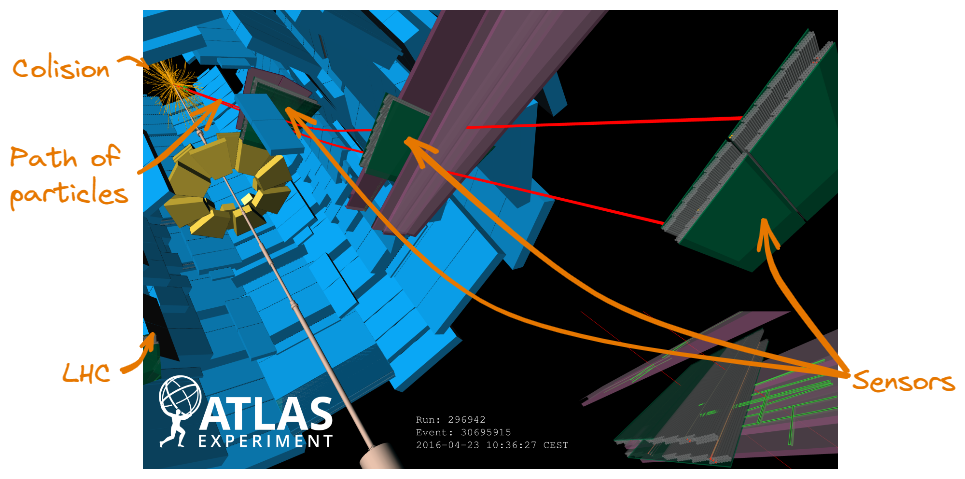
\includegraphics[width=0.85\textwidth]{05-resources/img/spec/experiment-atlas.excalidraw.png}
    \caption{ATLAS experiment at CERN~\cite{atlas-experiment}}
    \label{spec:fig:context:physics-simulation:lhc}
\end{figure}


\section{Lawrence Berkeley National Laboratory}
\label{spec:ch:context:lbl}

The \acrfull{lbl} is a national laboratory in Berkeley, California.
It is managed and operated by the University of California for the \acrfull{doe}.
The lab is situated in the hills of Berkeley and it is composed of many buildings and has a beautiful view of the San Francisco Bay (see Fig.\ref{spec:fig:context:lbl:lab-view}).

\begin{figure}[ht]
    \centering
    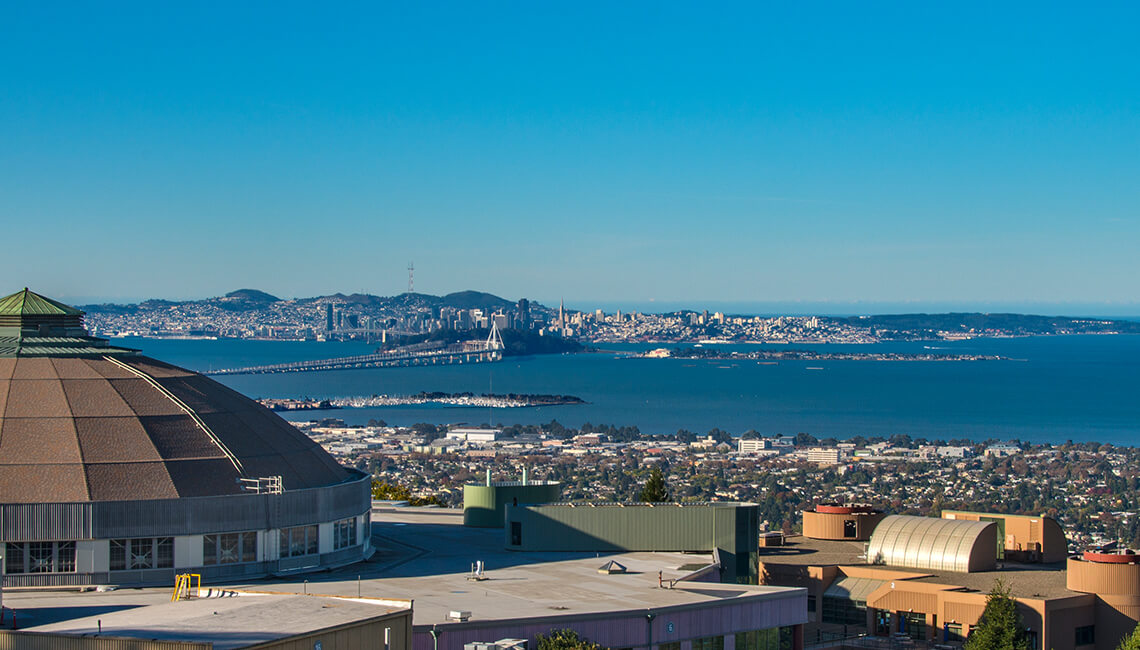
\includegraphics[width=0.8\textwidth]{05-resources/img/spec/lab-view.jpg}
    \caption{Lawrence Berkeley National Laboratory}
    \label{spec:fig:context:lbl:lab-view}
\end{figure}


The Physics and X-Ray Science Group, where the project is done, is situated in building 50f and the LBL ATLAS group, who are the customers of this project, are located in building 50.


\section{The Need}
\label{spec:ch:context:need}

Celeritas is already accelerated by \acrshort{gpu}s, however, the team wants to improve the performance to be able to reduce the time of a simulation.
In the current version of the code, each particle track is processed in parallel by one GPU thread, with no collaboration between threads.
GPU profiling of the code shows that execution time is dominated by two kernels.
The first one is handled by the interaction with the detector geometry to know where, in 3D space, the particle is situated and during the profiling, the library used is vecGeom~\cite{VecGeom}.
The second kernel, which will be the focus of this bachelor thesis project, is the computation of a differential equation using Dormand-Prince~\cite{princeDormand}.

\chapter{Goals}
\label{spec:ch:goals}

-

\chapter{Activities}
\label{spec:ch:activities}

Activities are all the tasks that need to be done to complete the project. These tasks
come directly from the goals. The planning is based on the activities listed above.

All the tasks aren't mentioning the documentation, but it's implicit that all the tasks will be reported in the final report.

\section{Learn GPU Programming}
\label{spec:ch:activities:learn-gpu-programming}

This step will launch the project and it can be without any knowledge of the project Celeritas, the objective is to learn the fundamentals of GPU programming.


\subsection{Learn CUDA}
\label{spec:ch:activities:learn-gpu-programming:learn-cuda}

First of all, the programming oriented \acrshort{gpu} and the language \acrshort{cuda} are totally new, there is no class about that in the bachelor program.

\acrlong{lbl} provide a course about CUDA~\cite{cuda-training} and some exercices~\cite{cuda-series} to learn the language. 


\subsection{Write cheat sheet}
\label{spec:spec:ch:activities:learn-gpu-programming:write-cheat-sheet}

For each course, a cheat sheet will be produced to summarize the important notions and provide quick access to the information during the realization of the project.
Not every course will produce a new one, a cheat sheet can be improved.


\section{Understand the project}
\label{spec:ch:activities:understand-the-project}
The first step to do in the laboratory is to understand the project and the code.


\subsection{Compile the code}
\label{spec:ch:activities:understand-the-project:compile-the-code}
Celeritas is made to be run on \acrshort{hpc} and it comes with a new tool to build it.
The first step is to understand the basis of Module~\cite{Module} and Spack~\cite{Spack} to be able to compile the code.
This task is the first one to do in the laboratory.


\subsection{Launch Job on Perlmutter}
\label{spec:ch:activities:understand-the-project:launch-job-on-perlmutter}
Perlmutter~\cite{Perlmutter} is the new \acrshort{hpc} of \acrshort{nersc}.
To launch a job on this kind of machine, it's not a simple command as on a personal computer.
This requires a script that includes some parameters and the command to launch the code.
This step must be done before launching the code.


\subsection{Profile the code}
\label{specspec:ch:activities:understand-the-project:profile-the-code}
To basis performance, in order to measure the improvement, the code must be profiled on Perlmutter.
This step includes launching the project and some basic knowledge of the Nvidia profiling tool.
It is very important to know the limit of the code and announce some objectives to reach before starting coding.
When a profile is recorded and analyzed, this will close the second goal of the project.


\subsection{Background the project}
\label{spec:ch:activities:understand-the-project:background-the-project}
Aside from the other task, this one will be done in order to understand the background of the project.
It is not mandatory to drive this bachelor thesis to success but it will help to understand what the other members of the team are doing and to provide a better view of the project in the final report.



\section{Improve the performance}
\label{spec:ch:activities:improve-the-performance}
This is the goal of this bachelor's thesis and to do that, several steps must be done to reach the objective.


\subsection{Understand the code}
\label{spec:ch:activities:improve-the-performance:understand-the-code}
First of all, it's important to understand how the code is working to not reinvent the wheel with a function that already exists.
The objective is also to follow the guideline of the project to make easier understanding and maintainability.


\subsection{Understand Runge-Kutta}
\label{spec:ch:activities:improve-the-performance:understand-runge-kutta}
As the optimization is on the Runge-Kutta method, it's important to understand how it's working and how it's implemented in the code.
Some analysis must be done to know where it's possible to improve the performance and how.


\subsection{Implement the optimization}
\label{spec:ch:activities:improve-the-performance:implement-the-optimization}
As all the analysis are done, it's time to implement a new version of the Runge-Kutta that use all the advantages of the \acrshort{gpu}.
This step will be done in several iterations to be sure that the code is working and that the performance are improved.



\chapter{Planning}
\label{spec:ch:planning}

To manage the projet, the project tool from GitHub will be used.
This allow to link code with issues that represent activities and add a better tracking of the project.
The planning is available on my personnal GitHub account~\cite{github-project}.

The following figure \ref{spec:fig:planning} show the planning of the project.
Normally, the bachelor thesis begin directly at the \acrshort{lbl} but due to the time required to get a visa, the plane has been delayed and the project has started in Switzerland.
The August 4th, the report need to be finished and sended to the \acrshort{heia} but the internship will continue until the end of August 11th.
This week will be use to finish the work on place and to present the work done to the team.
Exceptionally, the bachelor's thesis end date can be delayed up to one week due to the disagrement to obtain a visa.

\begin{figure}[ht]
    \centering
    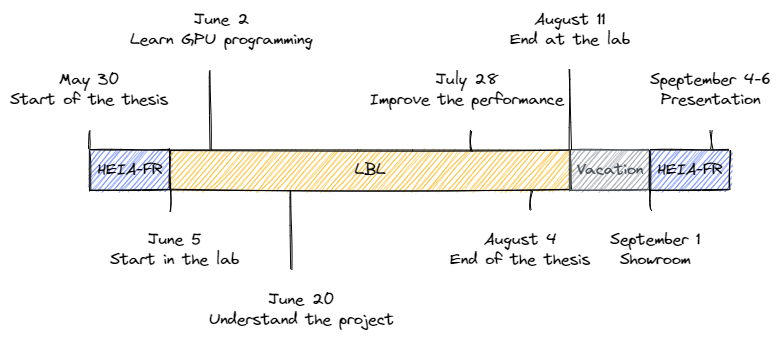
\includegraphics[width=\textwidth]{05-resources/img/spec/planning.excalidraw.png}
    \caption{Planning}
    \label{spec:fig:planning}
\end{figure}

The 1st september, there is a showroom at the \acrshort{heia} where all the student will present their work.
The final presentation will held between the 4th and the 7th september.

\section{Milestones}
\label{spec:ch:planning:milestones}

The milestones represent the main steps of the project.
The mandatory objectives can be found in the milestones.
They are used to track the progress of each step and set a list of activities to do.


\section{Issues}
\label{spec:ch:planning:issues}

The issues are representing the tasks that need to be done to complete a milestone.
They can be detailed with a checklist to specify the steps to follow and they can be linked to a pull request to keep a reference to the code that solves the issue.



% Appendices
% \appendix

% -----------------------------------------------------------------------------
% Back matter
% -----------------------------------------------------------------------------
% \backmatter

% List of figures
%\cleardoublepage
\phantomsection
\addcontentsline{toc}{chapter}{List of Figures}
\listoffigures
%\addcontentsline{toc}{chapter}{List of Tables}
%\listoftables

% Bibliography
%\cleardoublepage
\printbibliography[title={References}, heading=bibintoc]

% Glossary
\glsaddall
\printglossary[type=\acronymtype, nonumberlist]

% Add your CV here if you want

\end{document}

